\documentclass[17pt, a1paper, landscape, margin=10mm, innermargin=8mm, blockverticalspace=6mm, colspace=8mm]{tikzposter}

% Packages
\usepackage{amsmath, amssymb}
\usepackage{tabularx}
\usepackage{booktabs}
\usepackage{colortbl}
\usepackage{xcolor}
\usepackage{graphicx}
\usepackage{tikz}
\usepackage{pgfplots}
\pgfplotsset{compat=1.18}
\usetikzlibrary{shapes.geometric, arrows.meta, positioning, calc}

% KIU and Lecture Color Palette
\definecolor{kiunavy}{RGB}{15, 45, 82}        % KIU Dark Blue Title Banner
\definecolor{kiulightblue}{RGB}{74, 144, 226}  % Light blue borders for text boxes
\definecolor{kiured}{RGB}{204, 41, 54}        % Red border for key equations
\definecolor{kiugreen}{RGB}{46, 125, 50}      % Green border for recommendation
\definecolor{kiuamber}{RGB}{217, 119, 6}      % Amber for Warning boxes
\definecolor{boxbg}{RGB}{255, 255, 255}       % Clean white box fill

\tikzposterlatexaffectionproofoff

\makeatletter
% Custom Titlestyle: Dark-blue banner matching KIU lecture style
\definetitlestyle{KIUBanner}{
    width=\TP@visibletextwidth, roundedcorners=6, linewidth=0pt, innersep=5mm,
    titletotopverticalspace=0mm, titletoblockverticalspace=6mm,
    titlegraphictotitledistance=0pt, titletextscale=1
}{
    \draw[fill=kiunavy, draw=none, rounded corners=\titleroundedcorners]
        (\titleposleft,\titleposbottom) rectangle (\titleposright,\titlepostop);
}

% Reusable Custom Block Styles
% 1. Standard Text Box (Light-blue border)
\defineblockstyle{TextBlock}{
    titlewidthscale=1, bodywidthscale=1, titleleft,
    titleoffsetx=0pt, titleoffsety=0pt, bodyoffsetx=0pt, bodyoffsety=0pt,
    bodyverticalshift=0pt, roundedcorners=6, linewidth=1.8pt,
    titleinnersep=3mm, bodyinnersep=4mm
}{
    \ifBlockHasTitle
        \draw[color=kiulightblue, fill=boxbg, rounded corners=\blockroundedcorners, line width=\blocklinewidth]
            (blockbody.south west) rectangle (blocktitle.north east);
        \draw[color=kiulightblue, fill=kiulightblue!14, rounded corners=\blockroundedcorners, line width=\blocklinewidth]
            (blocktitle.south west) rectangle (blocktitle.north east);
    \else
        \draw[color=kiulightblue, fill=boxbg, rounded corners=\blockroundedcorners, line width=\blocklinewidth]
            (blockbody.south west) rectangle (blockbody.north east);
    \fi
}

% 2. Key Equation Box (Red border)
\defineblockstyle{EqBlock}{
    titlewidthscale=1, bodywidthscale=1, titleleft,
    titleoffsetx=0pt, titleoffsety=0pt, bodyoffsetx=0pt, bodyoffsety=0pt,
    bodyverticalshift=0pt, roundedcorners=6, linewidth=2.4pt,
    titleinnersep=3mm, bodyinnersep=4mm
}{
    \ifBlockHasTitle
        \draw[color=kiured, fill=kiured!2, rounded corners=\blockroundedcorners, line width=\blocklinewidth]
            (blockbody.south west) rectangle (blocktitle.north east);
        \draw[color=kiured, fill=kiured!15, rounded corners=\blockroundedcorners, line width=\blocklinewidth]
            (blocktitle.south west) rectangle (blocktitle.north east);
    \else
        \draw[color=kiured, fill=kiured!2, rounded corners=\blockroundedcorners, line width=\blocklinewidth]
            (blockbody.south west) rectangle (blockbody.north east);
    \fi
}

% 3. Recommendation Box (Green border)
\defineblockstyle{RecBlock}{
    titlewidthscale=1, bodywidthscale=1, titleleft,
    titleoffsetx=0pt, titleoffsety=0pt, bodyoffsetx=0pt, bodyoffsety=0pt,
    bodyverticalshift=0pt, roundedcorners=6, linewidth=2.4pt,
    titleinnersep=3mm, bodyinnersep=4.5mm
}{
    \ifBlockHasTitle
        \draw[color=kiugreen, fill=kiugreen!3, rounded corners=\blockroundedcorners, line width=\blocklinewidth]
            (blockbody.south west) rectangle (blocktitle.north east);
        \draw[color=kiugreen, fill=kiugreen!16, rounded corners=\blockroundedcorners, line width=\blocklinewidth]
            (blocktitle.south west) rectangle (blocktitle.north east);
    \else
        \draw[color=kiugreen, fill=kiugreen!3, rounded corners=\blockroundedcorners, line width=\blocklinewidth]
            (blockbody.south west) rectangle (blockbody.north east);
    \fi
}

% Patch internal \block title font to bold 24pt and body font to 15.5pt
\expandafter\patchcmd\csname\string\block\endcsname{\bf \LARGE}{\bfseries\fontsize{24pt}{28pt}\selectfont\color{kiunavy}}{}{}
\expandafter\patchcmd\csname\string\block\endcsname{\large}{\fontsize{15.5pt}{19.5pt}\selectfont}{}{}
\makeatother

\usetheme{Simple}
\usetitlestyle{KIUBanner}

% Custom Warning Box macro in lecture style
\newcommand{\warningbox}[2]{%
\vspace{0.25em}%
\noindent\begin{tikzpicture}%
\node[draw=kiuamber, line width=1.4pt, fill=kiuamber!8, rounded corners=4pt, inner sep=6pt, text width=\dimexpr\linewidth-16pt\relax, align=left] {%
  \textbf{\color{kiuamber!95!black}\normalsize Warning: #1}\par\vspace{0.15em}%
  {\small #2}%
};%
\end{tikzpicture}%
\vspace{0.25em}%
}

% Custom UPDR Cycle Icon (lecture style)
\newcommand{\updrbox}[4]{%
\begin{tikzpicture}[scale=0.82, baseline=-0.3ex]
  \tikzset{
    box/.style={draw=black!55, line width=0.8pt, rounded corners=2pt, minimum width=0.88cm, minimum height=0.52cm, font=\bfseries\footnotesize, align=center},
    active/.style={fill=blue!30, text=blue!95!black, draw=blue!85!black, line width=1.3pt},
    inactive/.style={fill=black!5, text=black!40}
  }
  \node[box, #1] (U) at (0, 0.36) {U};
  \node[box, #2] (P) at (0.95, 0.36) {P};
  \node[box, #3] (D) at (0.95, -0.26) {D};
  \node[box, #4] (R) at (0, -0.26) {R};
  \draw[->, >=stealth, line width=1.0pt, blue!75!black] (0.475, 0.05) ++(50:0.25cm) arc (50:390:0.25cm);
\end{tikzpicture}%
}
\newcommand{\updrU}{\updrbox{active}{inactive}{inactive}{inactive}}
\newcommand{\updrP}{\updrbox{inactive}{active}{inactive}{inactive}}
\newcommand{\updrD}{\updrbox{inactive}{inactive}{active}{inactive}}
\newcommand{\updrR}{\updrbox{inactive}{inactive}{inactive}{active}}

% Header Configuration
\settitle{
  \begin{minipage}[c]{0.18\linewidth}
    \vspace{0.1em}
    \fcolorbox{white}{white}{
\includegraphics[height=3.2cm, keepaspectratio]{kiu_logo.png}}
  \end{minipage}%
  \hfill
  \begin{minipage}[c]{0.58\linewidth}
    \centering
    \color{white}
    {\fontsize{28pt}{32pt}\bfseries Case 6: How Fast Should a Delivery Driver Drive? \par}
    \vspace{0.25em}
    {\fontsize{16pt}{20pt}\bfseries Cruising Speed Policy for Regional Fleets Under Energy vs.\ Time Trade-Offs \par}
    \vspace{0.2em}
    {\small Kutaisi International University \quad\textbar\quad Industry Case Studies: Solving Real Problems with Mathematics \par}
  \end{minipage}%
  \hfill
  \begin{minipage}[c]{0.25\linewidth}
    \raggedleft
    \color{white}
    {\small \textbf{Polya Steps 1--4 Industrial Problem Canvas} \par}
    \vspace{0.2em}
    {\footnotesize \textbf{Group 6:} Saba Dumbadze, Saba Tchitchinadze, Tato Diasamidze \par}
    \vspace{0.15em}
    {\footnotesize October 2026 \quad\textbar\quad Prof.\ Dr.\ Florian Rupp \par}
  \end{minipage}
}

\title{Case 6: How Fast Should a Delivery Driver Drive?}
\author{Group 6: Saba Dumbadze, Saba Tchitchinadze, Tato Diasamidze}
\institute{Kutaisi International University}

\begin{document}
\maketitle

\begin{columns}

% =========================================================================
% COLUMN 1: Sections A & B (Industrial Situation + Polya Step 1 Understand)
% =========================================================================
\column{0.33}
\useblockstyle{TextBlock}

% --- Block A: Industrial Situation ---
\block{Industrial Situation: The Operational Decision}{
  A regional delivery company wants drivers to finish long motorway sections quickly. Driving faster saves paid driver time but uses more fuel or electricity, and slower driving does the opposite. The operations manager must give drivers one recommended cruising speed.
  
  \vspace{0.25em}
  \noindent\textbf{The Decision Stated Precisely:}
  \textit{Which cruising speed $v$ should the company recommend on long motorway sections, and under which conditions (energy price, urgency, vehicle, route length) does this recommendation change?}

  \vspace{0.45em}
  % Input -> Model -> Output Diagram with Opposing Arrows
  \centering
  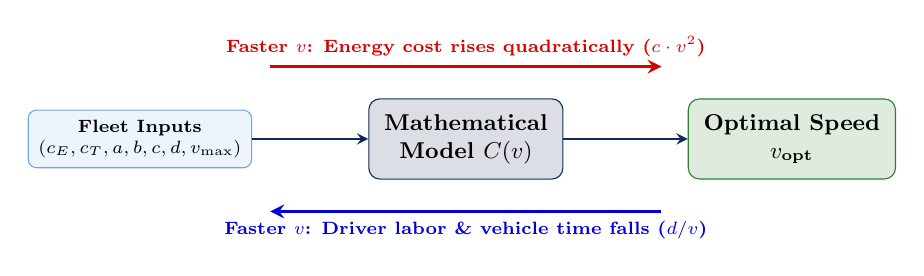
\begin{tikzpicture}[
    scale=0.92, every node/.style={transform shape},
    inbox/.style={draw=kiulightblue!80, fill=kiulightblue!10, rounded corners=3pt, font=\scriptsize\bfseries, align=center, inner sep=4pt},
    modbox/.style={draw=kiunavy, fill=kiunavy!15, rounded corners=4pt, font=\small\bfseries, align=center, inner sep=6pt},
    outbox/.style={draw=kiugreen, fill=kiugreen!15, rounded corners=4pt, font=\small\bfseries, align=center, inner sep=6pt},
    arr/.style={->, >=stealth, thick, color=kiunavy}
  ]
    \node[inbox] (inp) at (0,0) {Fleet Inputs\\$(c_E, c_T, a, b, c, d, v_{\max})$};
    \node[modbox] (mod) at (4.5,0) {Mathematical\\Model $C(v)$};
    \node[outbox] (out) at (9.0,0) {Optimal Speed\\$v_{\text{opt}}$};

    \draw[arr] (inp) -- (mod);
    \draw[arr] (mod) -- (out);

    % Opposing trade-off arrows
    \draw[->, >=stealth, very thick, red!85!black] (1.8, 1.0) -- (7.2, 1.0)
      node[midway, above, font=\scriptsize\bfseries, text=red!85!black] {Faster $v$: Energy cost rises quadratically ($c \cdot v^2$)};
    \draw[<-, >=stealth, very thick, blue!85!black] (1.8, -1.0) -- (7.2, -1.0)
      node[midway, below, font=\scriptsize\bfseries, text=blue!85!black] {Faster $v$: Driver labor \& vehicle time falls ($d/v$)};
  \end{tikzpicture}
}

% --- Block B: Polya Step 1 Understand ---
\block{\updrU\quad Step A: Understand (Industrial Problem Canvas)}{
  Mapped systematically onto the lecture's Problem Canvas fields (Slide 51):
  
  \vspace{0.2em}
  \begin{itemize}
    \setlength{\itemsep}{2.5pt}
    \setlength{\parskip}{0pt}
    \item \textbf{A.1 Situation:} Fleet operations dispatching vehicles across long, uniform motorway sections.
    \item \textbf{A.2 Problem:} Operational conflict between saving productive driver hours and paying for aerodynamic energy waste.
    \item \textbf{A.3 Decision:} Determine optimal cruising speed $v$ and quantify sensitivity across operational parameters.
    \item \textbf{A.4 Stakeholders:} Operations manager (decision maker), drivers (workload, safety), finance (energy expenses), customers (delivery arrival), maintenance (wear), sustainability officer, regulator (speed limits).
    \item \textbf{A.5 Success (Objective):} Minimize total operational route cost $C(v)$ while strictly meeting delivery deadlines.
    \item \textbf{A.6 Known Information:} Transit distance $d = 300\text{ km}$, functional form of vehicle energy $E(v)$, current energy prices.
    \item \textbf{A.7 Unknown Information:} Physical vehicle parameters ($a, b, c$), true value of driver time $c_T$, wear and liability costs.
    \item \textbf{A.8 Assumptions:} Constant speed, flat motorway, calm weather, unpriced wear absorbed into maximum legal threshold $v_{\max}$.
    \item \textbf{A.9 Hypothesis H1:} Minimizing energy alone is not sensible ($v_E \approx 42\text{ km/h}$ is far below usable motorway speeds).
    \item \textbf{A.9 Hypothesis H2:} At realistic values of time ($c_T > 6.3\text{ EUR/h}$), time cost dominates, pushing optimal speed to $v_{\max} = 110\text{ km/h}$.
    \item \textbf{A.9 Hypothesis H3:} An interior optimum exists only below a critical $\mu^*$, and is insensitive to parameter errors (cube-root law).
    \item \textbf{A.9 Hypothesis H4:} Longer routes need a lower optimal speed (tested \& refuted in Step 4).
    \item \textbf{A.10 Variables:} Decision: cruising speed $v$. Observables: trip time $T(v)$, energy $E(v)$. Uncertainties: $a, b, c, c_E, c_T$.
  \end{itemize}

  \warningbox{The wage is not the value of time.}{Saved driver time only possesses true economic value if the delivery schedule can productively utilize the saved minutes.}
}

% --- Block B2: Operational Parameters & Model Assumptions ---
\useblockstyle{TextBlock}
\block{Operational Parameters \& Model Simplifications}{
  \renewcommand{\arraystretch}{0.95}
  \centering
  \small
  \begin{tabularx}{0.98\linewidth}{l l l X}
    \toprule
    \textbf{Symbol} & \textbf{Physical Unit} & \textbf{Benchmark (Range)} & \textbf{Physical Meaning / Source Authority} \\
    \midrule
    $v$ & km/h & 70--130 & Decision variable; set by driver / fleet policy \\
    $d$ & km & 300 (150--500) & Route motorway transit distance (Dispatcher) \\
    $c_E$ & EUR/kWh & 0.25 (0.18--0.38) & Electricity contract tariff (Commercial energy market) \\
    $c_T$ & EUR/h & 20.0 (5--35) & Opportunity value of driver time (Wage + Urgency) \\
    $a, b, c$ & [phys. units] & 30, 450, $3.0\cdot 10^{-3}$ & Aeromechanical drag and rolling coefficients (OEM) \\
    $v_{\max}, T_{\max}$ & km/h, h & 110 km/h, 3.0 h & Highway speed limit code \& delivery deadline (SLA) \\
    \bottomrule
  \end{tabularx}
  
  \vspace{0.35em}
  \raggedright\small
  \textbf{Evaluation of Initial Model Simplifications (Canvas B.1):}
  \begin{itemize}
    \setlength{\itemsep}{2pt}
    \setlength{\parskip}{0pt}
    \item \textbf{Constant Speed:} Realistic on open motorway corridors; transient ramp and queue accelerations are negligible over long 300 km transits.
    \item \textbf{Flat Corridor:} Standard macroscopic fleet assumption; rolling elevation grades cancel out symmetrically across round-trips via regenerative braking.
    \item \textbf{Calm Atmospheric Conditions:} Neglects stochastic headwind/tailwind velocities; headwind $w$ shifts effective drag to $c(v+w)^2$, slightly lowering $v^*$.
    \item \textbf{Linear Time Cost:} Time value enters linearly ($c_T d/v$); step-penalty surcharges for missed deadlines are enforced via $T(v) \le T_{\max}$.
    \item \textbf{Fleet Homogeneity:} Uniform vehicle coefficients; mixed fleets require calibrated $(a_i, b_i, c_i)$ per vehicle class.
  \end{itemize}
}


% =========================================================================
% COLUMN 2: Sections C & D (Polya Step 2 Plan + Polya Step 3 Do)
% =========================================================================
\column{0.34}

% --- Block C: Step B Plan (Canvas Fields B.1 to B.8) ---
\useblockstyle{TextBlock}
\block{\updrP\quad Step B: Plan (Industrial Problem Canvas)}{
  Mapped systematically onto the lecture's Problem Canvas fields (Slide 53):
  
  \vspace{0.15em}
  \begin{itemize}
    \setlength{\itemsep}{2pt}
    \setlength{\parskip}{0pt}
    \item \textbf{B.1 Simplification:} Focus on steady cruising; isolate rolling resistance ($a$), auxiliary loads ($b/v$), and aerodynamic drag ($c\,v^2$). Initially ignore acceleration transients.
    \item \textbf{B.2 First Model:} 1D continuous convex cost: $C(v) = c_E(a + b/v + c\,v^2) + c_T(d/v)$, with travel time $T(v) = d/v$.
    \item \textbf{B.3 Mathematical Toolbox:} Calculus for optimum ($C'(v)=0, C''(v)>0$), boundary checking ($v \le v_{\max}$), sensitivity elasticity $\frac{\mu}{v^*}\frac{dv^*}{d\mu}$. \textit{Do not select a tool simply because we know it} (Slide 32).
    \item \textbf{B.4 Data (Needed vs.\ Have):} Have: physical vehicle model structure and benchmark parameters. Need: calibrated fleet consumption data before rollout.
    \item \textbf{B.5 Validation:} Verify limiting case ($\lim_{\mu \to 0} v^* = v_E$), ensure strict global convexity ($C''(v) > 0$), check feasibility against motorway speed limits.
    \item \textbf{B.6 Project Road-map:} Work packages: Model formulation $\rightarrow$ Analytical optimization $\rightarrow$ Constraint enforcement $\rightarrow$ Scenario evaluation $\rightarrow$ Actionable policy.
    \item \textbf{B.7 Time \& Effort Allocation:} Prioritize economic interpretation and management decision rules over unnecessary simulation.
    \item \textbf{B.8 Stop Criterion:} Closed-form analytical formula for $v^*$ and critical threshold $\mu^*$, answering the operations manager's question across all operating regimes.
  \end{itemize}
}

% --- Block D: Step C Do (Key Equations in Red Box - Canvas Fields C.1 to C.4) ---
\useblockstyle{EqBlock}
\block{\updrD\quad Step C: Do (Implementation \& Calculations)}{
  \noindent\textbf{The Exactly Five Governing Equations (Implementation C.1):}
  \begin{align}
    C(v) &= c_E \left(a + \frac{b}{v} + c\,v^2\right) + c_T \frac{d}{v} \label{eq:cost} \\
    v^* &= \left[\frac{c_E b + c_T d}{2 c_E c}\right]^{1/3} = \left[\frac{b + \mu d}{2c}\right]^{1/3} \label{eq:vstar} \\
    C(v^* + \delta) - C(v^*) &\approx 3\,c_E c\,\delta^2 \label{eq:curv} \\
    \frac{\mu}{v^*}\frac{dv^*}{d\mu} &= \frac{1}{3}\frac{\mu d}{b + \mu d} \le \frac{1}{3} \label{eq:elast} \\
    \mu^* &= \frac{2c\,v_{\max}^3 - b}{d} \implies v_{\text{opt}} = \begin{cases} v^* & \mu < \mu^* \\ v_{\max} & \mu \ge \mu^* \end{cases} \label{eq:mu}
  \end{align}

  \vspace{-0.2em}
  \noindent\textbf{Documented Benchmark Parameters (C.2, $d = 300\text{ km}$, Electric Van):}\\
  $a = 30\text{ kWh}$, $b = 450\text{ kWh}\cdot\text{km/h}$, $c = 3.0\cdot 10^{-3}\text{ kWh}\cdot\text{h}^2/\text{km}^2$, $c_E = 0.25\text{ EUR/kWh}$, $v_{\max} = 110\text{ km/h}$, $T_{\max} = 3\text{ h}$.
  
  \vspace{0.15em}
  \noindent\textbf{Plausibility Checks \& Comparisons (C.3 \& C.4):} Energy-minimal baseline $v_E = (b/(2c))^{1/3} \approx 42.2\text{ km/h}$ (confirms H1). Critical operating threshold $\mu^* = (2c v_{\max}^3 - b)/d \approx 25.1\text{ kW} \implies c_T^* \approx 6.27\text{ EUR/h}$.
  
  \vspace{0.3em}
  % Scenario Comparison Table
  \centering
  \small
  \renewcommand{\arraystretch}{1.0}
  \begin{tabularx}{0.98\linewidth}{l X X}
    \toprule
    \textbf{Speed} & \textbf{Scenario 1: $c_T = 20\text{ EUR/h}$ (Standard)} & \textbf{Scenario 2: $c_T = 5\text{ EUR/h}$ (Low Urgency)} \\
    \midrule
    $70\text{ km/h}$  & 98.50 EUR (+37\%) & 34.21 EUR (+10\%) \\
    $90\text{ km/h}$  & 81.49 EUR (+13\%) & 31.49 EUR (+1.2\%) \\
    $100\text{ km/h}$ & 76.13 EUR (+5.5\%) & 31.13 EUR (+0.05\%) \\
    $110\text{ km/h}$ & \textbf{72.14 EUR (Best, limit binds)} & 31.23 EUR (+0.4\%) \\
    $v^* = 102.4\text{ km/h}$ & N/A ($v^* = 159.7$, clamped at 110) & \textbf{31.11 EUR (Best interior)} \\
    \bottomrule
  \end{tabularx}

  \vspace{0.4em}
  % Two Side-by-Side Publication-Grade Plots using PGFPlots
  \begin{minipage}{0.49\linewidth}
    \centering
    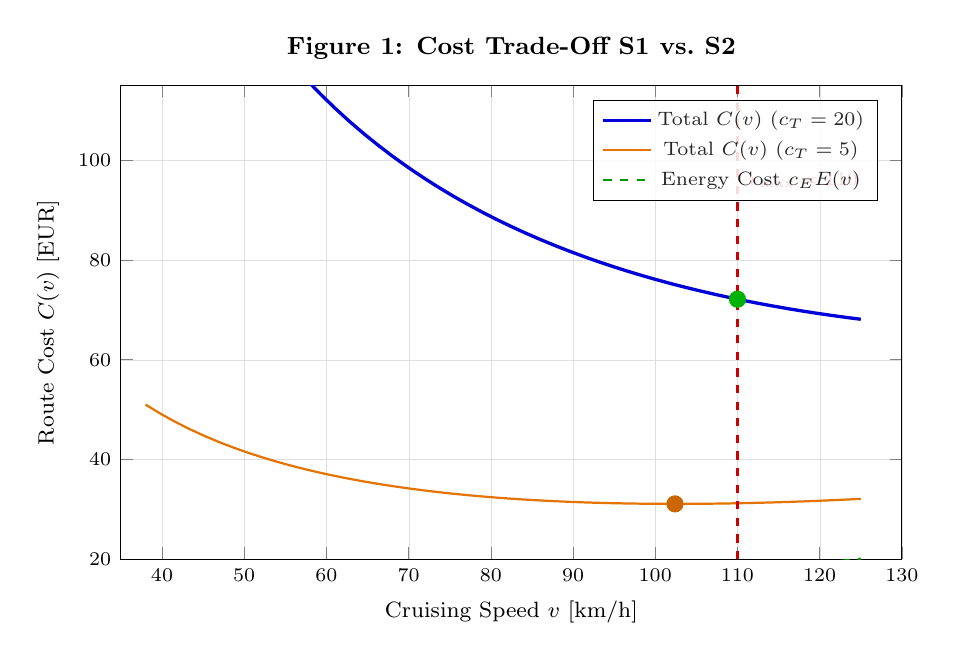
\begin{tikzpicture}
      \begin{axis}[
        title={\textbf{Figure 1: Cost Trade-Off S1 vs.\ S2}},
        title style={font=\small\bfseries},
        width=11.5cm, height=7.6cm,
        xlabel={\footnotesize Cruising Speed $v$ [km/h]},
        ylabel={\footnotesize Route Cost $C(v)$ [EUR]},
        xmin=35, xmax=130, ymin=20, ymax=115,
        grid=both, grid style={line width=.1pt, draw=gray!25},
        legend pos=north east, legend style={font=\scriptsize, fill=white, fill opacity=0.85},
        tick label style={font=\scriptsize}
      ]
        % S1 Cost: c_T = 20
        \addplot[domain=38:125, samples=50, blue!85!black, very thick] {0.25*(30 + 450/x + 0.003*x^2) + 20*300/x};
        \addlegendentry{Total $C(v)$ ($c_T=20$)}
        % S2 Cost: c_T = 5
        \addplot[domain=38:125, samples=50, orange!90!black, thick] {0.25*(30 + 450/x + 0.003*x^2) + 5*300/x};
        \addlegendentry{Total $C(v)$ ($c_T=5$)}
        % Energy Cost component
        \addplot[domain=38:125, samples=40, green!60!black, dashed, thick] {0.25*(30 + 450/x + 0.003*x^2)};
        \addlegendentry{Energy Cost $c_E E(v)$}
        % v_max vertical line
        \draw[red!80!black, dashed, line width=1.1pt] (axis cs:110, 20) -- (axis cs:110, 115)
          node[pos=0.8, right, font=\scriptsize, text=red!80!black] {$v_{\max}=110$};
        % Recommended point
        \node[circle, fill=green!70!black, inner sep=2.2pt] at (axis cs:110, 72.14) {};
        \node[circle, fill=orange!80!black, inner sep=2.2pt] at (axis cs:102.4, 31.11) {};
      \end{axis}
    \end{tikzpicture}
  \end{minipage}%
  \hfill
  \begin{minipage}{0.49\linewidth}
    \centering
    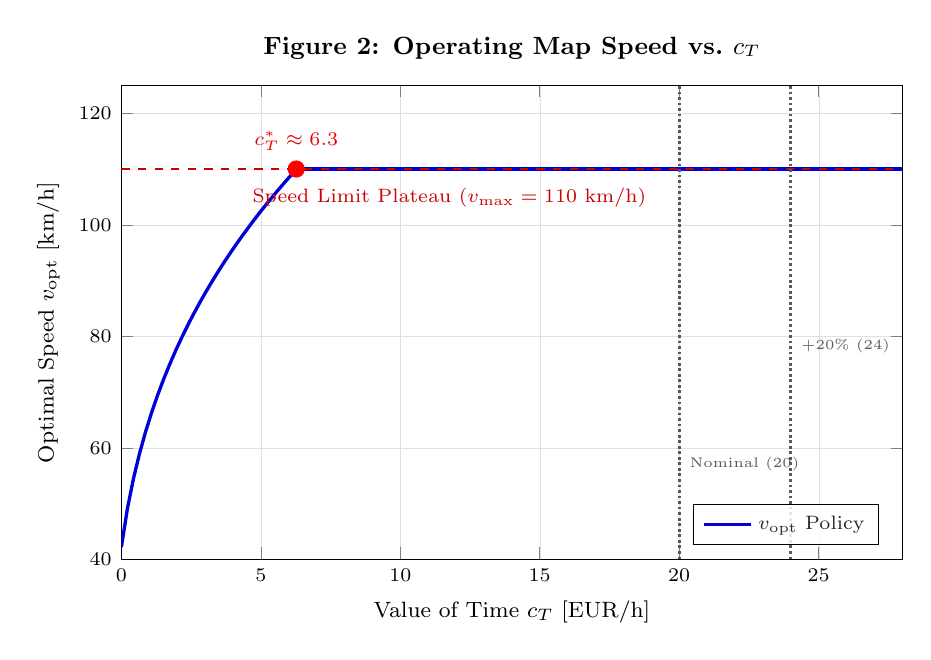
\begin{tikzpicture}
      \begin{axis}[
        title={\textbf{Figure 2: Operating Map Speed vs.\ $c_T$}},
        title style={font=\small\bfseries},
        width=11.5cm, height=7.6cm,
        xlabel={\footnotesize Value of Time $c_T$ [EUR/h]},
        ylabel={\footnotesize Optimal Speed $v_{\text{opt}}$ [km/h]},
        xmin=0, xmax=28, ymin=40, ymax=125,
        grid=both, grid style={line width=.1pt, draw=gray!25},
        legend pos=south east, legend style={font=\scriptsize, fill=white, fill opacity=0.85},
        tick label style={font=\scriptsize}
      ]
        % v_opt curve: min(((450 + (x/0.25)*300)/0.006)^(1/3), 110)
        \addplot[domain=0:6.27, samples=30, blue!85!black, very thick] {((450 + (x/0.25)*300)/0.006)^(1/3)};
        \addlegendentry{$v_{\text{opt}}$ Policy}
        \addplot[domain=6.27:28, samples=20, blue!85!black, very thick] {110};
        % Plateau limit line
        \draw[red!80!black, dashed, line width=1.0pt] (axis cs:0, 110) -- (axis cs:28, 110)
          node[pos=0.42, below=3pt, font=\scriptsize, text=red!80!black] {Speed Limit Plateau ($v_{\max} = 110\text{ km/h}$)};
        % Critical point
        \node[circle, fill=red, inner sep=2.2pt] at (axis cs:6.27, 110) {};
        \node[above=3pt, font=\scriptsize, text=red!90!black] at (axis cs:6.27, 110) {$c_T^* \approx 6.3$};
        % Current value and +20%
        \draw[gray!70!black, densely dotted, line width=1.0pt] (axis cs:20, 40) -- (axis cs:20, 125)
          node[pos=0.2, right, font=\tiny] {Nominal (20)};
        \draw[gray!70!black, densely dotted, line width=1.0pt] (axis cs:24, 40) -- (axis cs:24, 125)
          node[pos=0.45, right, font=\tiny] {+20\% (24)};
      \end{axis}
    \end{tikzpicture}
  \end{minipage}
}


% =========================================================================
% COLUMN 3: Sections E, F, Symbols, AI & Sources
% =========================================================================
\column{0.33}

% --- Block E: Polya Step 4 Reflect (Canvas Fields D.1 to D.8) ---
\useblockstyle{TextBlock}
\block{\updrR\quad Step D: Reflect (Industrial Problem Canvas)}{
  Mapped systematically onto the lecture's Problem Canvas fields (Slide 55):
  
  \vspace{0.15em}
  \begin{itemize}
    \setlength{\itemsep}{2.5pt}
    \setlength{\parskip}{0pt}
    \item \textbf{D.1 Mathematical Verification:} First derivative yields closed-form root $v^* = [(b+\mu d)/(2c)]^{1/3}$. Second derivative $C''(v^*) = 6 c_E c > 0$ strictly guarantees global uniqueness. Limiting case $\lim_{\mu \to 0} v^* = v_E \approx 42.2\text{ km/h}$.
    \item \textbf{D.2 Real-World Validation (Hypotheses):}
      \begin{itemize}
        \setlength{\itemsep}{1pt}
        \item \textit{H1 (Energy Minimum):} Supported. $v_E \approx 42\text{ km/h}$ is dangerously slow and legally prohibited on motorways.
        \item \textit{H2 (Wage Dominance):} Supported. Commercial wages ($15\text{--}25\text{ EUR/h} > 6.3\text{ EUR/h}$) place operations on the $v_{\max}$ limit plateau.
        \item \textit{H3 (Flat Curvature):} Supported. Interior optimum exists only for low time-value ($\mu < \mu^*$). Flat curvature ($3 c_E c \delta^2$) renders costs highly forgiving to small speed deviations ($\pm 5\text{ km/h} \implies < 0.1\%$ cost increase).
        \item \textit{H4 (Route Length):} Refuted. Route length $d$ scales energy and time proportionally, leaving optimal cruising speed $v^*$ independent of $d$.
      \end{itemize}
    \item \textbf{D.3 Robustness:} Cost is flat near $v^*$. Parameter sensitivity: drag $c +20\%$ shifts $v^*$ down by only $-5.9\%$ (factor $1.2^{-1/3}$). Time cost $c_T +20\%$ shifts $v^*$ by at most $+6.3\%$.
    \item \textbf{D.4 Limitations:} Unpriced battery wear and traffic risk (handled via $v_{\max}$ ceiling), constant gradient, no traffic congestion shocks.
    \item \textbf{D.5 Interpretation:} Answers Slide 49's core question: \textit{What changed? What matters? What should the fleet manager do on Monday morning?}
    \item \textbf{D.7 Confidence:} High confidence for motorway cruising; speed limit $v_{\max}$ provides a safe operational upper bound.
    \item \textbf{D.8 Next Steps:} Calibrate coefficients $a,b,c$ from physical vehicle test runs before full fleet rollout.
  \end{itemize}

  \warningbox{Optimal speed $\neq$ Fastest speed $\neq$ Most energy-efficient speed.}{True cost optimality balances energy expenditure against productive labor utility.}
  
  \warningbox{Better fit $\neq$ Better model (Slides 36--45).}{High-degree regression without aeromechanical basis produces unphysical non-convexities.}

  \vspace{0.2em}
  % Closing Lecture Strip
  \begin{center}
  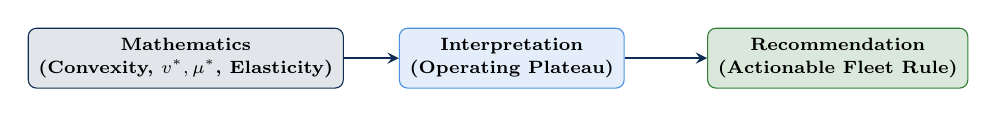
\begin{tikzpicture}[scale=0.92, every node/.style={transform shape}]
    \node[draw=kiunavy, fill=kiunavy!12, rounded corners=3pt, font=\scriptsize\bfseries, inner sep=4pt, align=center] (m) at (0,0) {Mathematics\\[0.1em](Convexity, $v^*, \mu^*$, Elasticity)};
    \node[draw=kiulightblue, fill=kiulightblue!15, rounded corners=3pt, font=\scriptsize\bfseries, inner sep=4pt, align=center] (i) at (4.5,0) {Interpretation\\[0.1em](Operating Plateau)};
    \node[draw=kiugreen, fill=kiugreen!18, rounded corners=3pt, font=\scriptsize\bfseries, inner sep=4pt, align=center] (r) at (9.0,0) {Recommendation\\[0.1em](Actionable Fleet Rule)};
    \draw[->, >=stealth, thick, kiunavy] (m) -- (i);
    \draw[->, >=stealth, thick, kiunavy] (i) -- (r);
  \end{tikzpicture}
  \end{center}
}

% --- Block F: Official Recommendation (Green Box - EXACT 66 WORDS) ---
\useblockstyle{RecBlock}
\block{D.6 Recommendation (Executive Policy for Monday Morning)}{
  \large\textbf{\color{kiugreen!90!black}Official Recommendation to Operations Management (Slide 49):}
  
  \vspace{0.3em}
  {\fontsize{16pt}{22pt}\selectfont\noindent\textit{``Drive at the legal limit (110 km/h) on long motorway sections whenever a saved driver-hour is worth more than about 6 EUR; at 20 EUR/h, driving 90 km/h instead raises route cost by about 13\%. If deliveries have slack, drive only as fast as the deadline requires. Slower speeds save energy but cost more in time. Replace our assumed consumption data by fleet measurements before rollout.''}}\par
  \vspace{0.2em}
  \hfill \footnotesize\textbf{(Exactly 66 words answering ``What should the company do on Monday morning?'')}
}

% --- Symbol Glossary (Task & Lecture Standards) ---
\useblockstyle{TextBlock}
\block{Notation, Physical Quantities \& Symbols}{
  \renewcommand{\arraystretch}{1.0}
  \centering
  \small
  \begin{tabularx}{0.98\linewidth}{l l X l l X}
    \toprule
    \textbf{Symbol} & \textbf{Unit} & \textbf{Physical Meaning / Role} & \textbf{Symbol} & \textbf{Unit} & \textbf{Physical Meaning / Role} \\
    \midrule
    $v$ & km/h & Cruising decision variable & $c_E$ & EUR/kWh & Energy electricity unit tariff \\
    $v^*$ & km/h & Unconstrained analytical optimum & $c_T$ & EUR/h & Opportunity value of driver time \\
    $d$ & km & Transit route distance & $\mu$ & kW & Time value in energy units ($c_T/c_E$) \\
    $T(v)$ & h & Motorway transit time ($d/v$) & $\mu^*$ & kW & Critical threshold where limit binds \\
    $E(v)$ & kWh & Route energy consumption & $C(v)$ & EUR & Total route operational cost \\
    \bottomrule
  \end{tabularx}
  
  \vspace{0.25em}
  \raggedright\footnotesize
  \textbf{Lecture Standard Clarification:} Following course conventions, $E$ denotes total route energy consumption (distinct from activation energy in Case 1); $T$ denotes transit travel time (distinct from reactor temperature in Case 1).
}

\end{columns}

\end{document}
